
\documentclass[11pt,a4paper]{report}
\usepackage{float}
\usepackage{tikz}
\usetikzlibrary{plotmarks}
\usepackage{amsmath,graphicx}
\usepackage{epstopdf}
\usepackage[font=normal,labelfont=bf]{caption}
\usepackage{subcaption}
\usepackage{color}
\usepackage[T1]{fontenc}
\usepackage{lmodern}
\usepackage{scalefnt}

% margin size
\usepackage[margin=1in]{geometry}
%\documentclass[border=2pt,tikz]{standalone}
\usetikzlibrary{positioning}

\newcommand{\scl}{0.06}

\begin{document}\tikzset{block/.style={node distance=-1pt, line width=1pt}}
\begin{tikzpicture}
\centering
 \node[block] (0) {\includegraphics[scale=\scl]{./subcortical_Test.png}};
       \node[block, below=of 0] (1) {\includegraphics[scale=\scl]{./cortical-inner-right-hemisphere_Test.png}};
       \node[block, below=of 1] (2) {\includegraphics[scale=\scl]{./cortical-outer-right-hemisphere_Test.png}};
      
    \node[block,above=of 0] {Test};
    \end{tikzpicture}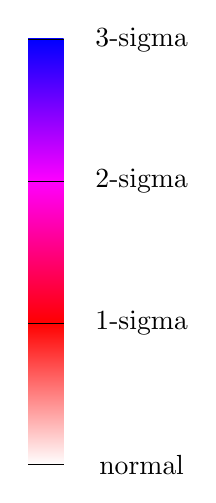
\begin{tikzpicture}[scale=0.9,auto,swap]
    \definecolor{color_0}{rgb}{1, 1, 1}
    \definecolor{color_1}{rgb}{1, 0, 0}
    \definecolor{color_2}{rgb}{1, 0, 1}
    \definecolor{color_3}{rgb}{0, 0, 1}
    \shade[bottom color=color_0,top color=color_1] (0,0) rectangle (0.5,2.01);
    
    \shade[bottom color=color_1,top color=color_2] (0,2) rectangle (0.5,4.01);
    
    \shade[bottom color=color_2,top color=color_3] (0,4) rectangle (0.5,6.01);
     
    \draw (0,0) -- (0.5,0);\node[inner sep=0] (corr_text) at (1.6,0.0) {normal};
       
    \draw (0,2) -- (0.5,2);\node[inner sep=0] (corr_text) at (1.6,2.0) {1-sigma};
       
    \draw (0,4) -- (0.5,4);\node[inner sep=0] (corr_text) at (1.6,4.0) {2-sigma};
       
    \draw (0,6) -- (0.5,6);\node[inner sep=0] (corr_text) at (1.6,6.0) {3-sigma};
      

  \end{tikzpicture}
  \end{document}